\section{Testing}

\subsection{Unit testing}
\subsection{Profiling}

\subsubsection{Profiling different \texttt{PriorityQueue} implementations}


After running the profiling experiments in the code, we have found that
problems with a fast growing queue generate a problematic space overhead, that
is translated to big garbage collection pauses that make execution slow. The
cost centers reveal that the space allocation happen most of all in the
\texttt{DataStructure} methods for adding nodes, so let us keep researching how
to fix this issue. To generate a lot of nodes in the open list, we will use a
bad heuristic in the problem \texttt{Warcraft}, to get a solution with these
statistics (obtained with the \texttt{Search.Monadic} library):

\begin{itemize}
 \item Number of expanded nodes: 378790
 \item Number of enqueued nodes: 734887
 \item Maximum length of the queue: 356099
\end{itemize}

Just to obtain a plan length of 19. This big size for the open list will
trigger the garbage collection problem and let us study it better. Running the
\texttt{profiling} executable of the library in this problem outputs, we can
see these results (please bear in mind the profiling overhead, stated as
\texttt{PROF} time):

\begin{lstlisting}
> cabal run profiling
   4,452,597,512 bytes allocated in the heap
   5,673,545,840 bytes copied during GC
     234,847,840 bytes maximum residency (45 sample(s))
       1,616,992 bytes maximum slop
             472 MB total memory in use (0 MB lost due to fragmentation)

                                     Tot time (elapsed)  Avg pause  Max pause
  Gen  0      8573 colls,     0 par    1.030s   1.050s     0.0001s    0.0004s
  Gen  1        45 colls,     0 par    7.107s   7.359s     0.1635s    0.3832s

  TASKS: 4 (1 bound, 3 peak workers (3 total), using -N1)

  SPARKS: 0 (0 converted, 0 overflowed, 0 dud, 0 GC'd, 0 fizzled)

  INIT    time    0.001s  (  0.010s elapsed)
  MUT     time    3.333s  (  5.247s elapsed)
  GC      time    6.249s  (  6.495s elapsed)
  RP      time    0.000s  (  0.000s elapsed)
  PROF    time    1.888s  (  1.914s elapsed)
  EXIT    time    0.003s  (  0.046s elapsed)
  Total   time   11.475s  ( 11.797s elapsed)

  Alloc rate    1,335,764,960 bytes per MUT second

  Productivity  29.1% of total user, 28.6% of total elapsed
\end{lstlisting}


We can see how the profiler returns that only a 29.1\% of the time has been
spent in actual search computations, while more than half of the execution time
(54.5\%) has been spent in garbage collection. To check if this space leak is
caused by our implementation or by the library used to implement the priority
queue, we can experiment with different methods.\\

We can run the same problem using the implementation with the \texttt{psqueues}
(and more accurately the \texttt{Data.IntPSQ} module), an alternative library
that offers an implementation of a higher level than our original \texttt{heap}
package. The results are as follow:


\begin{lstlisting}
> cabal run profiling
   4,867,074,880 bytes allocated in the heap
   4,823,508,568 bytes copied during GC
     183,851,592 bytes maximum residency (46 sample(s))
       1,405,912 bytes maximum slop
             373 MB total memory in use (0 MB lost due to fragmentation)

                                     Tot time (elapsed)  Avg pause  Max pause
  Gen  0      9345 colls,     0 par    0.992s   1.017s     0.0001s    0.0018s
  Gen  1        46 colls,     0 par    5.654s   5.849s     0.1271s    0.2936s

  TASKS: 4 (1 bound, 3 peak workers (3 total), using -N1)

  SPARKS: 0 (0 converted, 0 overflowed, 0 dud, 0 GC'd, 0 fizzled)

  INIT    time    0.001s  (  0.012s elapsed)
  MUT     time    3.508s  (  4.884s elapsed)
  GC      time    5.292s  (  5.498s elapsed)
  RP      time    0.000s  (  0.000s elapsed)
  PROF    time    1.354s  (  1.367s elapsed)
  EXIT    time    0.003s  (  0.037s elapsed)
  Total   time   10.159s  ( 10.431s elapsed)

  Alloc rate    1,387,545,376 bytes per MUT second

  Productivity  34.6% of total user, 34.1% of total elapsed
\end{lstlisting}


There, it can be seen that the garbage collection time has been reduced by a
second, but it is still a marginal improvement. Therefore, maybe a different
approach is needed: If we take a close look to the \texttt{addList} method, the
main cost center of this problem, we can see that we have two main options to
implement it: the first of them is to create a new \texttt{MinPrioHeap} and use
the library function \texttt{union} to merge both of them inside the new
structure. The code is shown in the listing \ref{addlist:union}.

\begin{lstlisting}[style=haskell, caption= \texttt{addList} using
  \texttt{union}, label=addlist:union]
addList xs (PriorityQueue h f) = PriorityQueue (union h xs') f
  where xs' = fromList $ map (\n -> (f n, n)) xs
\end{lstlisting}

Although the language should manage the memory correctly, maybe this is not the
best way of managing this operation. As a possible solution, we can try to
force the reutilization of the old structure by adding the nodes using a strict
fold over the \texttt{MinPrioHeap}. This implementation is shown in the listing
\ref{addlist:fold}.

\begin{lstlisting}[style=haskell, caption= \texttt{addList} using
  \texttt{fold'}, label=addlist:fold]
addList xs (PriorityQueue h f) = PriorityQueue (foldl' insertNode h xs) f
  where insertNode acc x = insert (f x, x) acc
\end{lstlisting}

To check the performance of all possibilities, the profiling problem stated at
the beginning of this subsection has been run using all combination of
implementations and library, and the full results of performance are found in
the chart shown in the figure X.\\

\begin{figure}
\centering
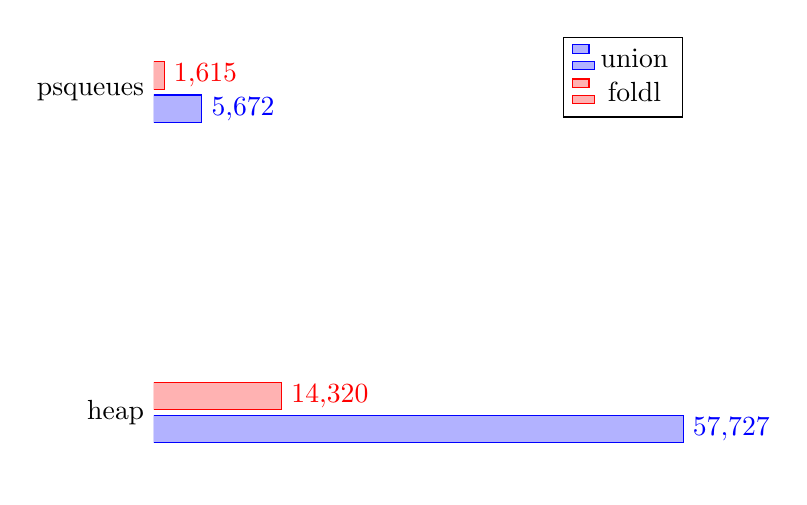
\begin{tikzpicture}
  \begin{axis}[
    xbar,
    y axis line style = { opacity = 0 },
    axis x line       = none,
    % width = 8cm, height = 4cm,
    ytick = data,
    tickwidth         = 0pt,
    enlarge y limits  = 0.2,
    enlarge x limits  = 0.02,
    symbolic y coords = {heap,psqueues},
    nodes near coords,
  ]
  \addplot coordinates { (57727,heap) (5672,psqueues) };
  \addplot coordinates { (14320,heap) (1615,psqueues) };
  \legend{union, foldl}
  \end{axis}
\end{tikzpicture}
\caption{Hello} \label{fig:f}
\end{figure}

\newpage